\documentclass[11pt]{article}
\usepackage{geometry}                % See geometry.pdf to learn the layout options. There are lots.
\geometry{letterpaper}                   % ... or a4paper or a5paper or ... 
%\geometry{landscape}                % Activate for for rotated page geometry
%\usepackage[parfill]{parskip}    % Activate to begin paragraphs with an empty line rather than an indent
\usepackage{graphicx}
\usepackage{amssymb}
\usepackage{amsmath}
\usepackage{epstopdf}
\usepackage{hyperref}
\usepackage{natbib}
\DeclareGraphicsRule{.tif}{png}{.png}{`convert #1 `dirname #1`/`basename #1 .tif`.png}


\graphicspath{
{/Users/Andy/Cruises_Research/Chipod/IO8S/}
{/Users/Andy/Cruises_Research/Chipod/IO8S/Figures/}
{/Users/Andy/Cruises_Research/ChiPod/IO8S/Data/proc/Chipod/SN1013/figures/}
{/Users/Andy/Cruises_Research/ChiPod/IO8S/Data/proc/Chipod/SN2001/figures/}
{/Users/Andy/Cruises_Research/ChiPod/IO8S/Data/proc/Chipod/SN2003/figures/}
{/Users/Andy/Cruises_Research/ChiPod/IO8S/Data/proc/Chipod/SN2002/figures/}
{/Users/Andy/Cruises_Research/ChiPod/IO8S/Data/proc/Chipod/SN2004/figures/}
{/Users/Andy/Cruises_Research/ChiPod/IO8S/Data/proc/Chipod/SN2020/figures/}
{/Users/Andy/Cruises_Research/ChiPod/IO8S/Data/proc/Chipod/SN2009/figures/}
}

\title{I08 CTD-Chipod Notes}
\author{Andy Pickering}
%\date{}                                           % Activate to display a given date or no date


\begin{document}
\maketitle

\tableofcontents
\newpage

%~~~~~~~~~~~~~~~~~~~~~~~~~~~~~
\section{About}

Notes on processing and analysis of CTD-chipod data collected during I08 cruise..

\begin{figure}[htbp]
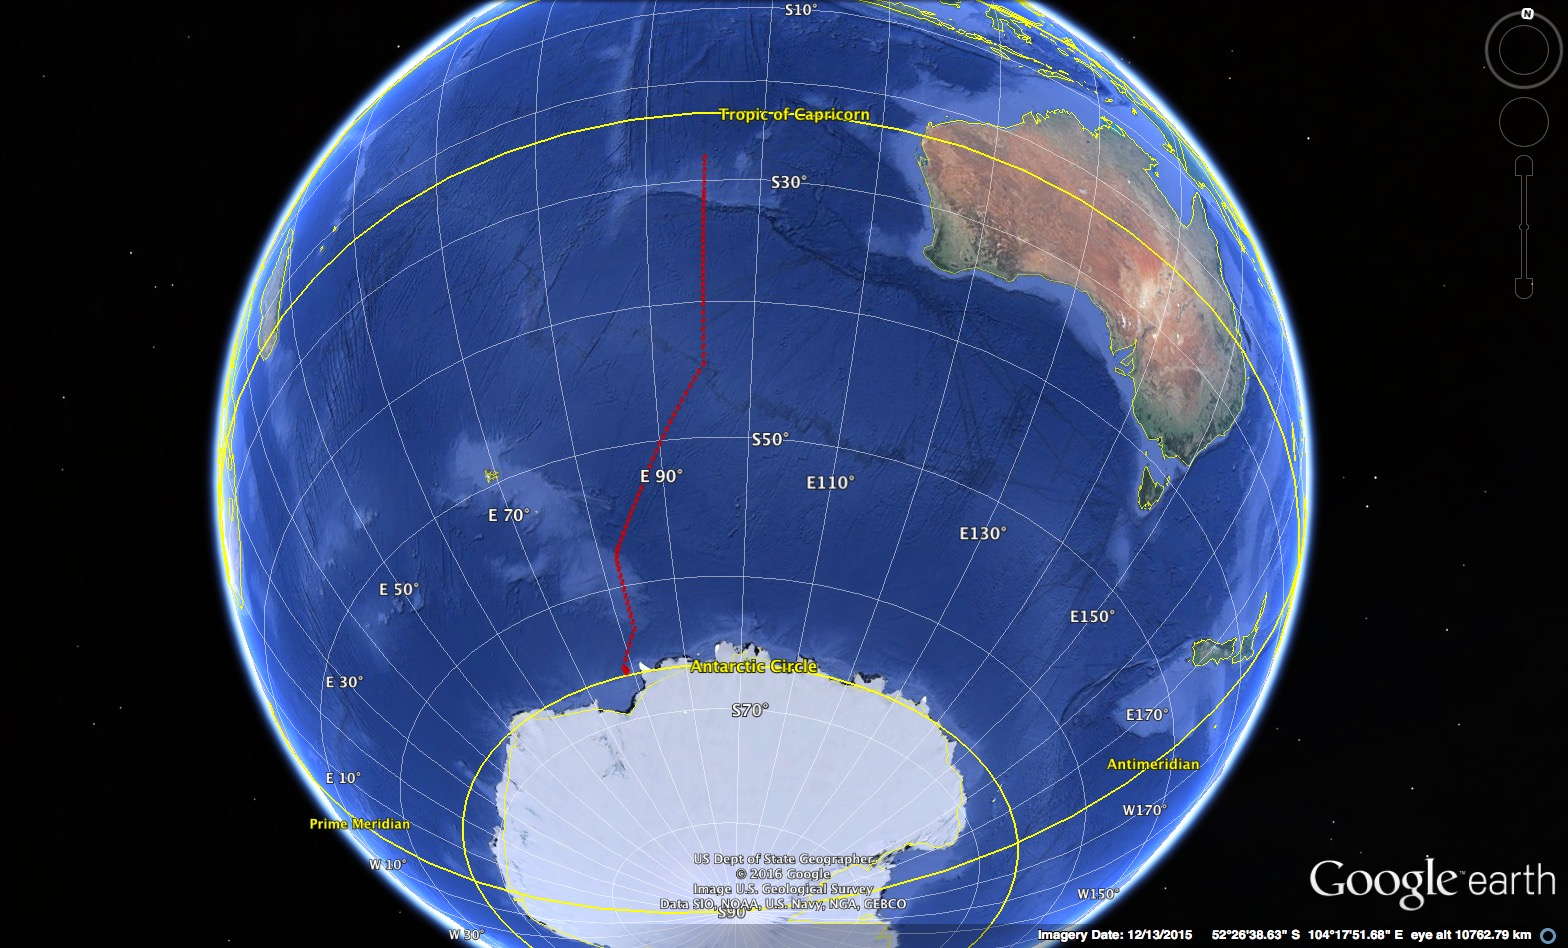
\includegraphics[width=38pc]{I08_kml_map.jpg}
\caption{Map of CTD cast locations during I08 cruise.}
\label{map}
\end{figure}


%~~~~~~~~~~~~~~~~~~~~~~~~~~~~~
\section{Data and Processing Outline}

Data paths are set w/ : 
\begin{itemize}
\item \verb+Load_chipod_paths_I08.m+
\end{itemize}

Chipod deployment info is given in 
\begin{itemize}
\item \verb+Chipod_Deploy_Info_I08+
\end{itemize}


%~~~~~~~~
\subsection{CTD}

Raw (hex) CTD data are processed with:
\begin{itemize}
\item \verb+Process_CTD_hex_I08.m+
\end{itemize}

%~~~~~~~~
\subsection{Chipod}

Raw chipod files are plotted with 
\begin{itemize}
\item \verb+PlotChipodDataRaw_I08.m+
\end{itemize}
to check for obvious issues/malfunctions with any of the instruments; these plots are saved in \verb+/Figures/chipodraw/+. Files with obviously bad or missing data (based on above raw plots) are noted in \verb+bad_file_list_I08.m+ and, which will prevent them from being loaded in the processing.

Processing scripts are:
\begin{itemize}
\item \verb+MakeCasts_CTDchipod_I08.m+
\item \verb+DoChiCalc_I08.m+
\end{itemize}

%~~~~~~~~
\subsection{Further processing and analysis}

\begin{itemize}
\item Data from all casts are combined into a single structure w/ \verb+MakeCombinedStructI08L.m+
\item 
\end{itemize}


\newpage
%~~~~~~~~~~~~~~~~~~~~~~~~~~~~~
\section{Processing Notes}

\begin{itemize}
\item Lost CTD package w/ chipods 2020, 2003, 2004, and 2001 early in cruise (near cast 10-15?).
\item Table \ref{chidepinfo} gives the info for $\chi$pods deployed.
\item Table \ref{procsum} gives a summary of the processing from MakeCasts.
\end{itemize}


\begin{table}[htdp]
\caption{$\chi$pod Deployment Info}
\begin{center}
\begin{tabular}{|c|c|c|c|}
\hline
SN & Type & Dir & Sensor \\ 
\hline
\hline
SN1013 & mini & up & 14-34D \\ 
SN2020 & mini & up & 14-28D \\ 
SN2014 & mini & up & 10-06MP \\ 
SN2009 & mini & up & 11-25D \\ 
SN2004 & mini & down & 13-02D \\ 
SN2003 & mini & up & 11-24D \\ 
SN2002 & mini & down & 13-05D \\ 
SN2001 & mini & down & 10-01MP \\ 
\hline
\end{tabular}
\end{center}
\label{chidepinfo}
\end{table}%

% table made in SummarizeProcIO8.m
\begin{table}[htdp]
\caption{Some $\chi$pod processing summary info for IO8S. There were 89 CTD casts.}
\begin{center}
\begin{tabular}{|c|c|c|c|}
\hline
SN & $\chi$ data & T1cal Good & toffset $<$ 1min \\ 
\hline
\hline
SN1013 & 59 & 56 & 57 \\ 
SN2020 & 11 & 0 & 10 \\ 
SN2014 & 0 & 0 & 0 \\ 
SN2009 & 59 & 57 & 57 \\ 
SN2004 & 10 & 2 & 9 \\ 
SN2003 & 8 & 1 & 8 \\ 
SN2002 & 50 & 43 & 49 \\ 
SN2001 & 10 & 6 & 9 \\ 
\hline
\end{tabular}
\end{center}
\label{procinfo}
\end{table}


\begin{figure}[htbp]
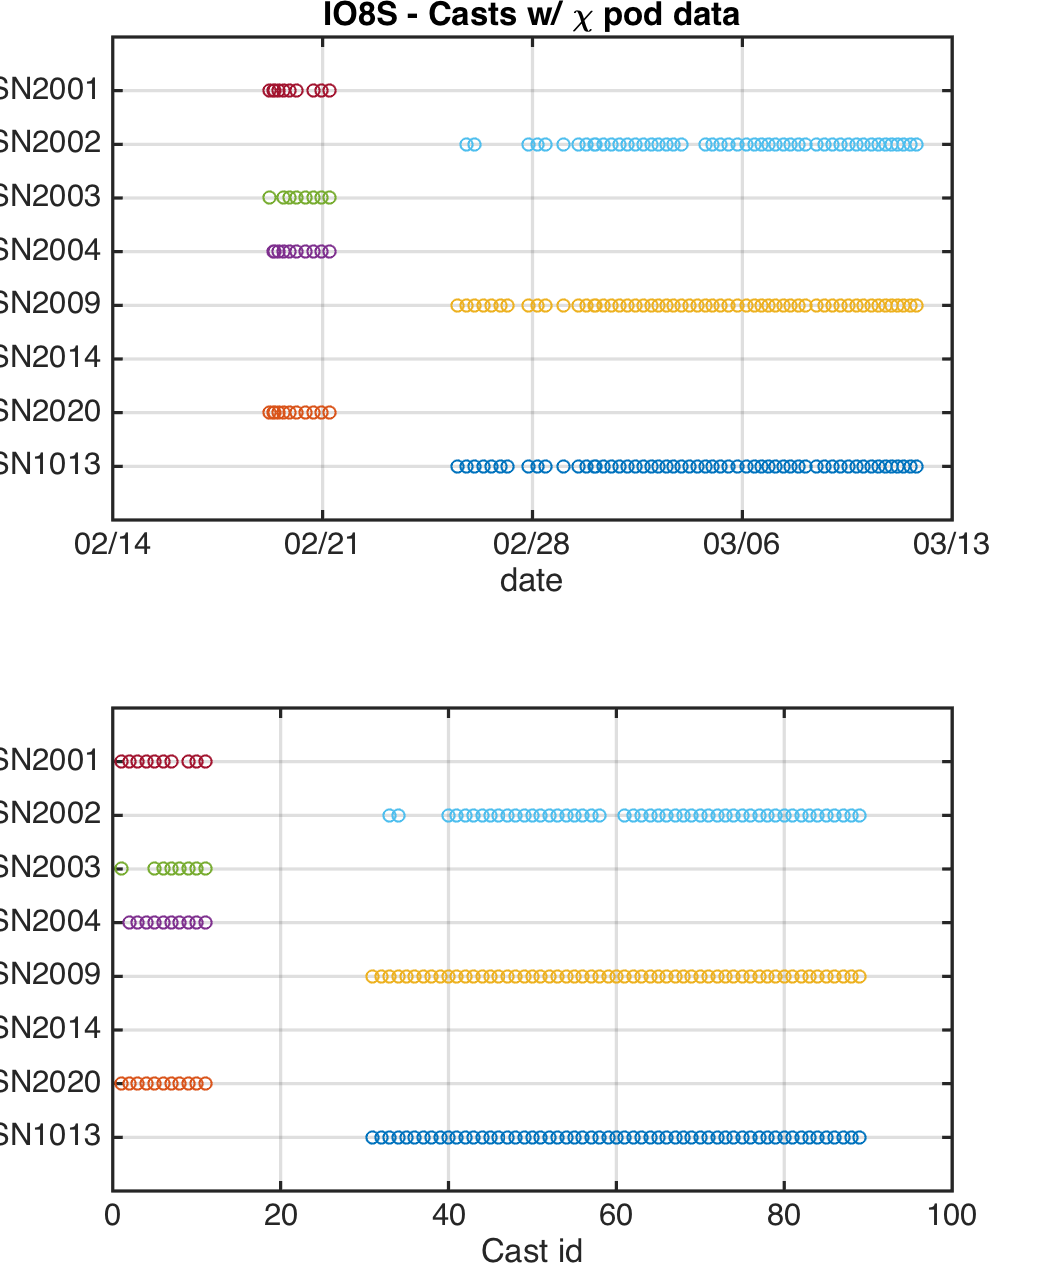
\includegraphics[scale=0.7]{IO8S_haveChiData_all.png}
\caption{Figure showing which casts there is $\chi$pod data for. Note castid is NOT necessarily same as cast numbers in CTD files.}
\label{ischidata}
\end{figure}


%~~
\subsubsection{Time Offsets}


\begin{figure}[htbp]
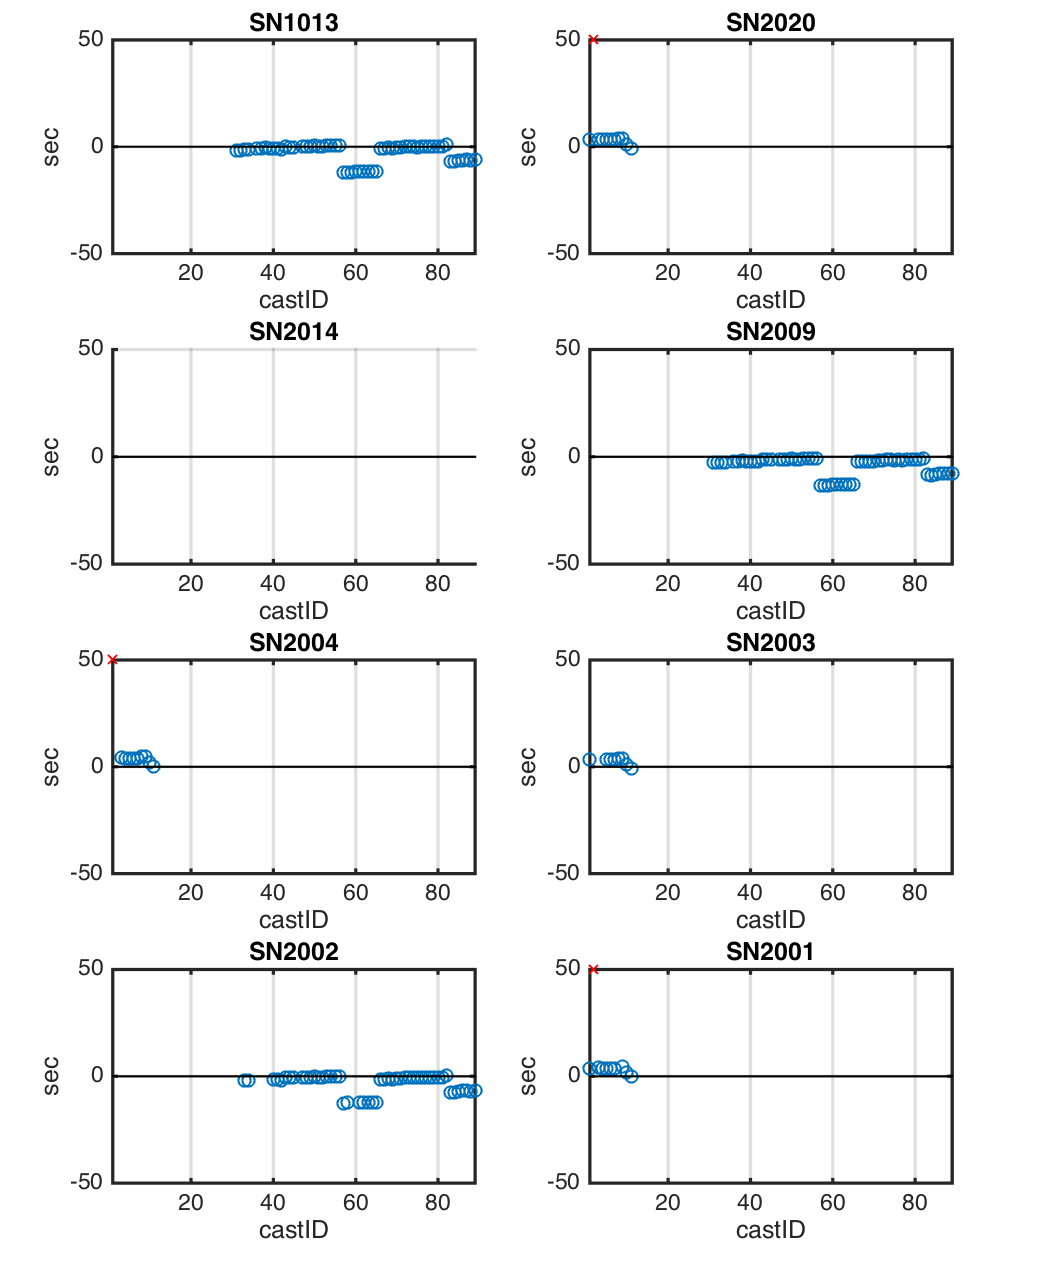
\includegraphics[scale=1]{IO8S_timeoffsets_all.png}
\caption{Time-offsets for all $\chi$pods, found by aligning with CTD data.}
\label{toffs}
\end{figure}


%~~~~~~~~~~~~~~~~~~~~~~~~~~~~~
\section{Example (raw) Chipod Data for 1 cast}

\begin{figure}[htbp]
\includegraphics[scale=0.7]{SN1013_03601_Fig1_RawChipodTS.png}
\caption{Raw chipod data from SN1013 for one CTD cast.}
\label{sn1013_1}
\end{figure}


\begin{figure}[htbp]
\includegraphics[scale=0.7]{SN2001_01001_Fig1_RawChipodTS.png}
\caption{Raw chipod data from SN2001 for a CTD cast.}
\label{sn2001_1}
\end{figure}

\begin{figure}[htbp]
\includegraphics[scale=0.7]{SN2002_03501_Fig1_RawChipodTS.png}
\caption{Raw chipod data from SN2002 for a CTD cast.}
\label{sn2002_1}
\end{figure}

\begin{figure}[htbp]
\includegraphics[scale=0.7]{SN2003_00702_Fig1_RawChipodTS.png}
\caption{Raw chipod data from SN2003 for a CTD cast.}
\label{sn2003_1}
\end{figure}

\begin{figure}[htbp]
\includegraphics[scale=0.7]{SN2004_00801_Fig1_RawChipodTS.png}
\caption{Raw chipod data from SN2004 for a CTD cast.}
\label{sn2004_1}
\end{figure}

\begin{figure}[htbp]
\includegraphics[scale=0.7]{SN2009_02801_Fig1_RawChipodTS.png}
\caption{Raw chipod data from SN2009 for a CTD cast.}
\label{sn2009_1}
\end{figure}

\begin{figure}[htbp]
\includegraphics[scale=0.7]{SN2020_00901_Fig1_RawChipodTS.png}
\caption{Raw chipod data from SN2020 for a CTD cast.}
\label{sn2020_1}
\end{figure}






\newpage
%~~~~~~~~~~~~~~~~~~~~~~~~~~~~~
\section{Results}





\clearpage
%~~
\section{Data from each individual Chipod}

%~~~~~~~
\subsection{SN1013}

\begin{figure}[htbp]
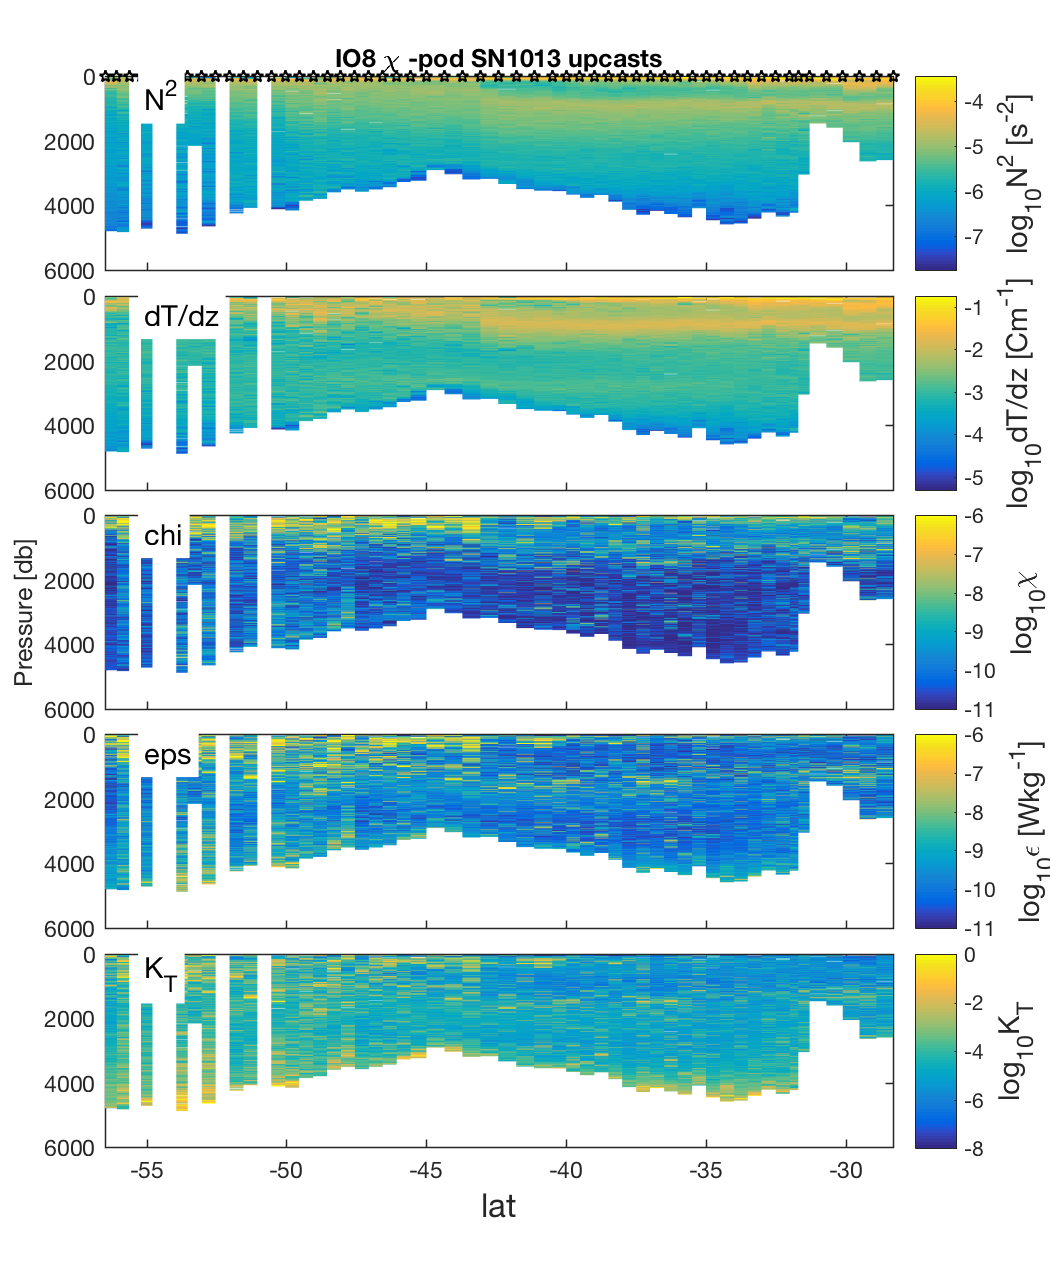
\includegraphics[scale=0.9]{XC_SN1013_Vs_lat_upAllVars.png}
\caption{All chipod profiles from sensor SN1013. Variables are: N2, dTdz, chi, eps, and KT.}
\label{}
\end{figure}

%~~~~~~~
\subsection{SN2001}
\begin{figure}[htbp]
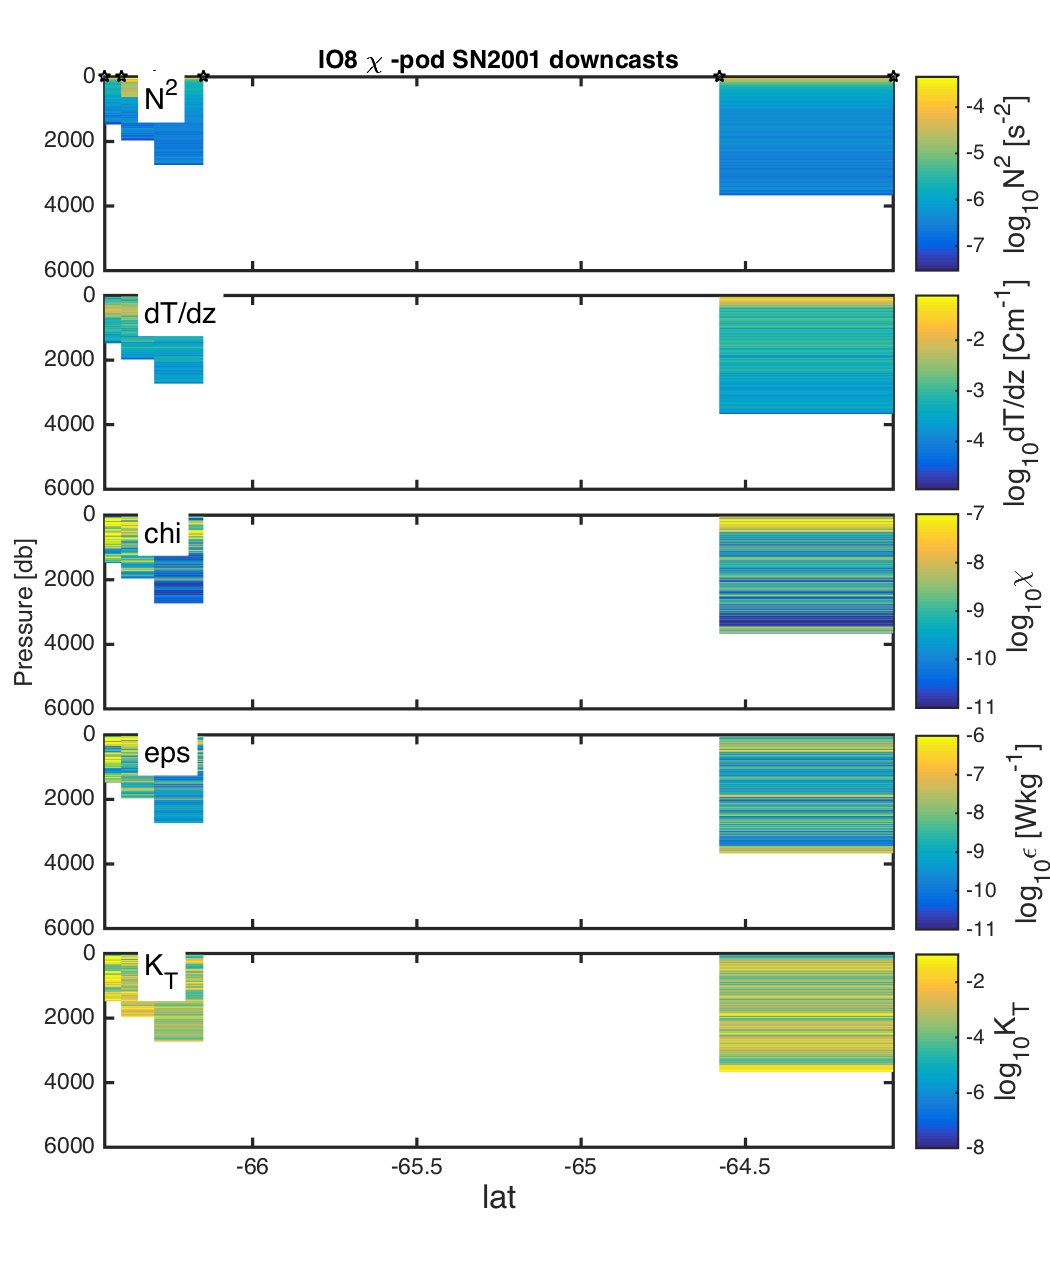
\includegraphics[scale=0.9]{XC_SN2001_Vs_lat_downAllVars.png}
\caption{All chipod profiles from sensor SN2001. Variables are: N2, dTdz, chi, eps, and KT.}
\label{}
\end{figure}

%~~~~~~~
\subsection{SN2002}

\begin{figure}[htbp]
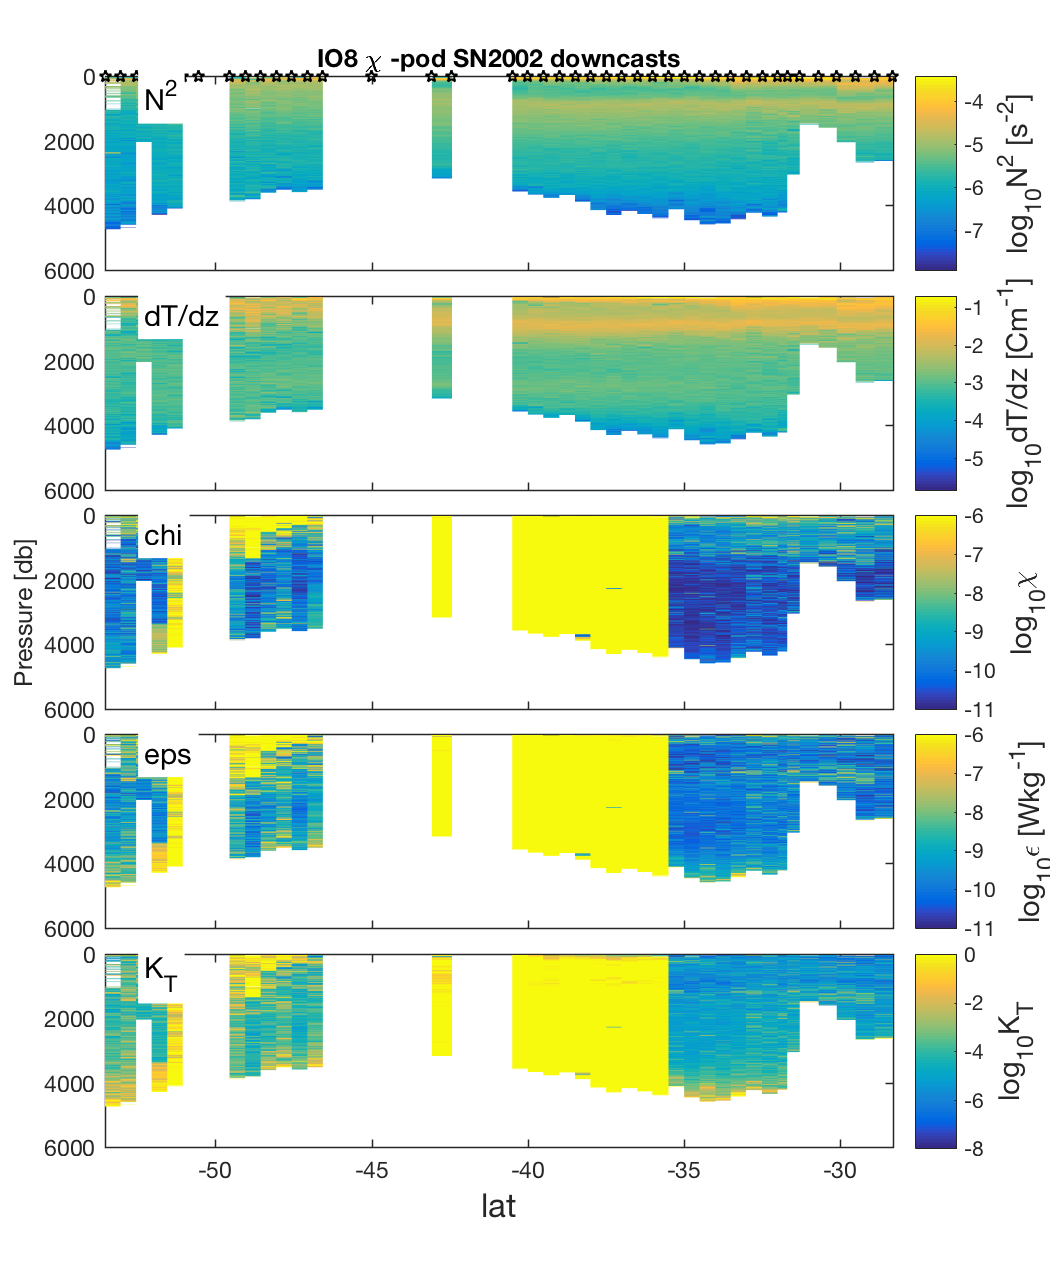
\includegraphics[scale=0.9]{XC_SN2002_Vs_lat_downAllVars.png}
\caption{All chipod profiles from sensor SN2002. Variables are: N2, dTdz, chi, eps, and KT.}
\label{}
\end{figure}

%~~~~~~~
\subsection{SN2003}

\begin{figure}[htbp]
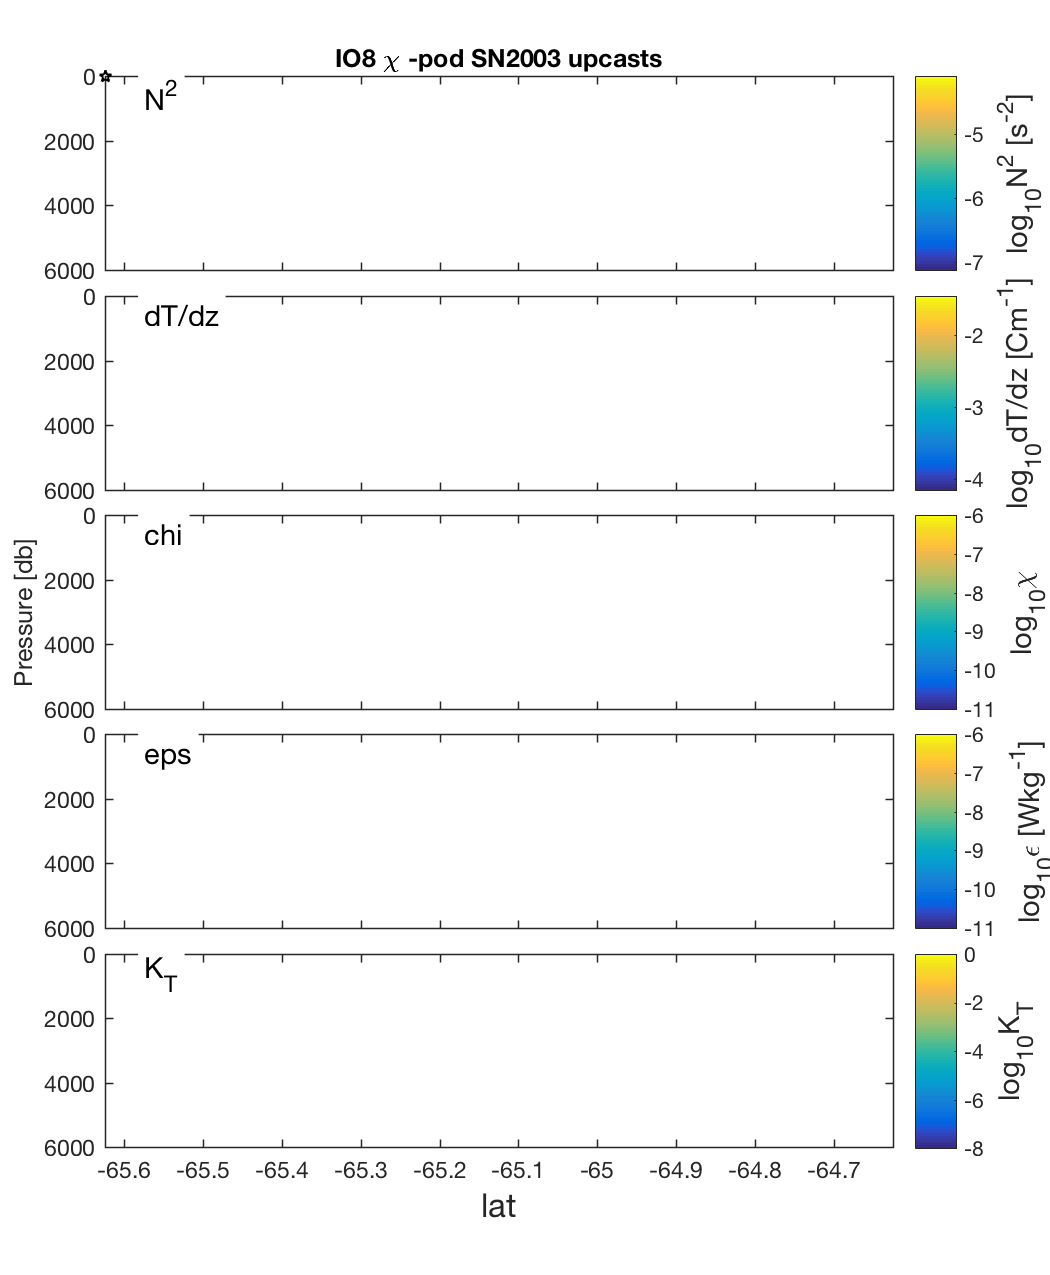
\includegraphics[scale=0.9]{XC_SN2003_Vs_lat_upAllVars.png}
\caption{All chipod profiles from sensor SN2003. Variables are: N2, dTdz, chi, eps, and KT.}
\label{}
\end{figure}

%~~~~~~~
\subsection{SN2004}

\begin{figure}[htbp]
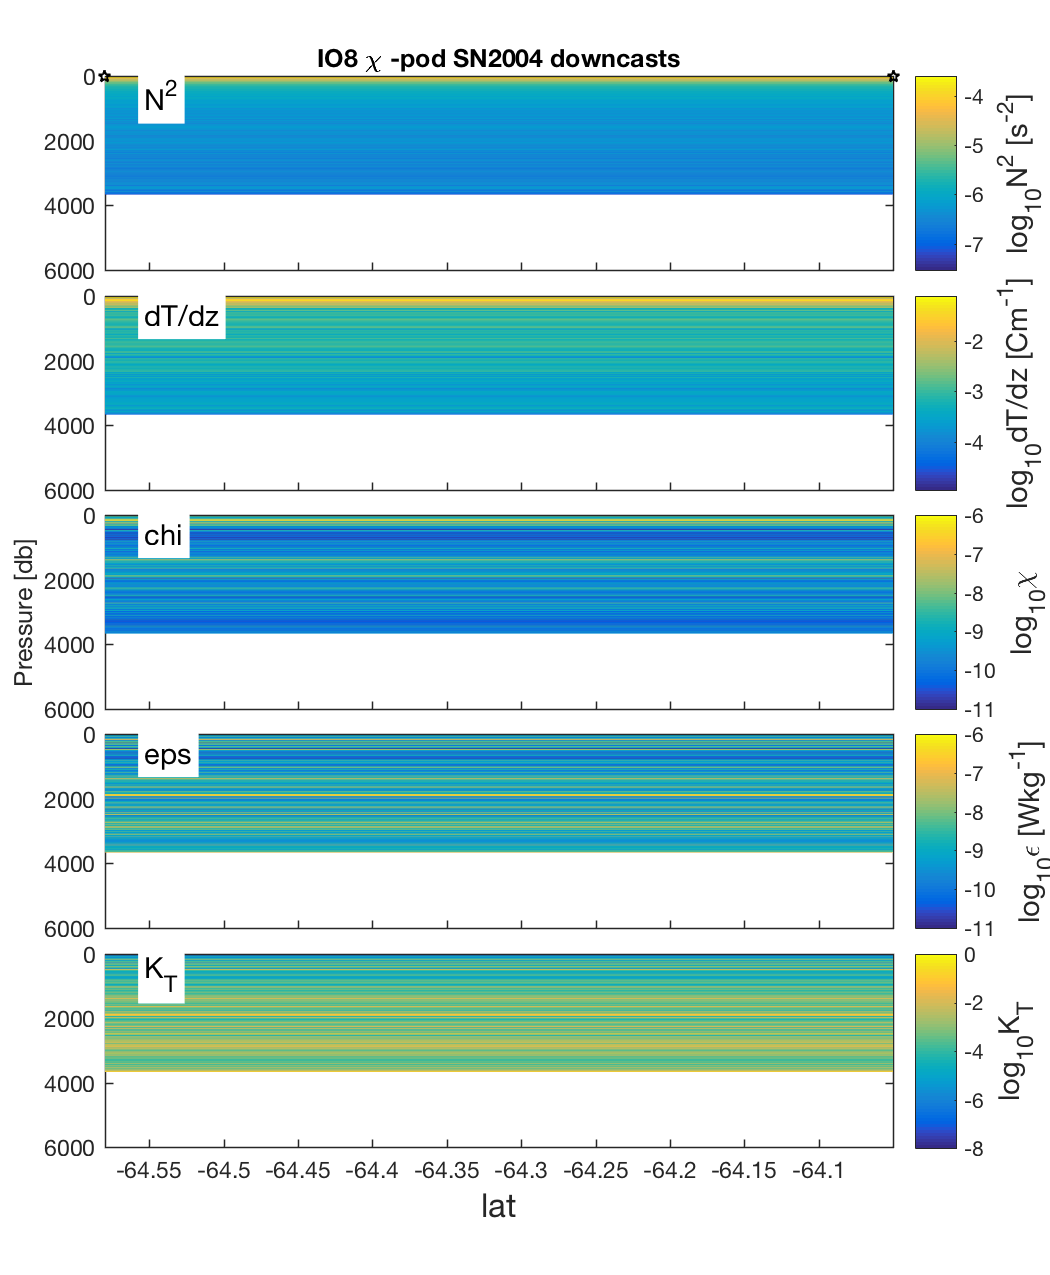
\includegraphics[scale=0.9]{XC_SN2004_Vs_lat_downAllVars.png}
\caption{All chipod profiles from sensor SN2004. Variables are: N2, dTdz, chi, eps, and KT.}
\label{}
\end{figure}

%~~~~~~~
\subsection{SN2009}

\begin{figure}[htbp]
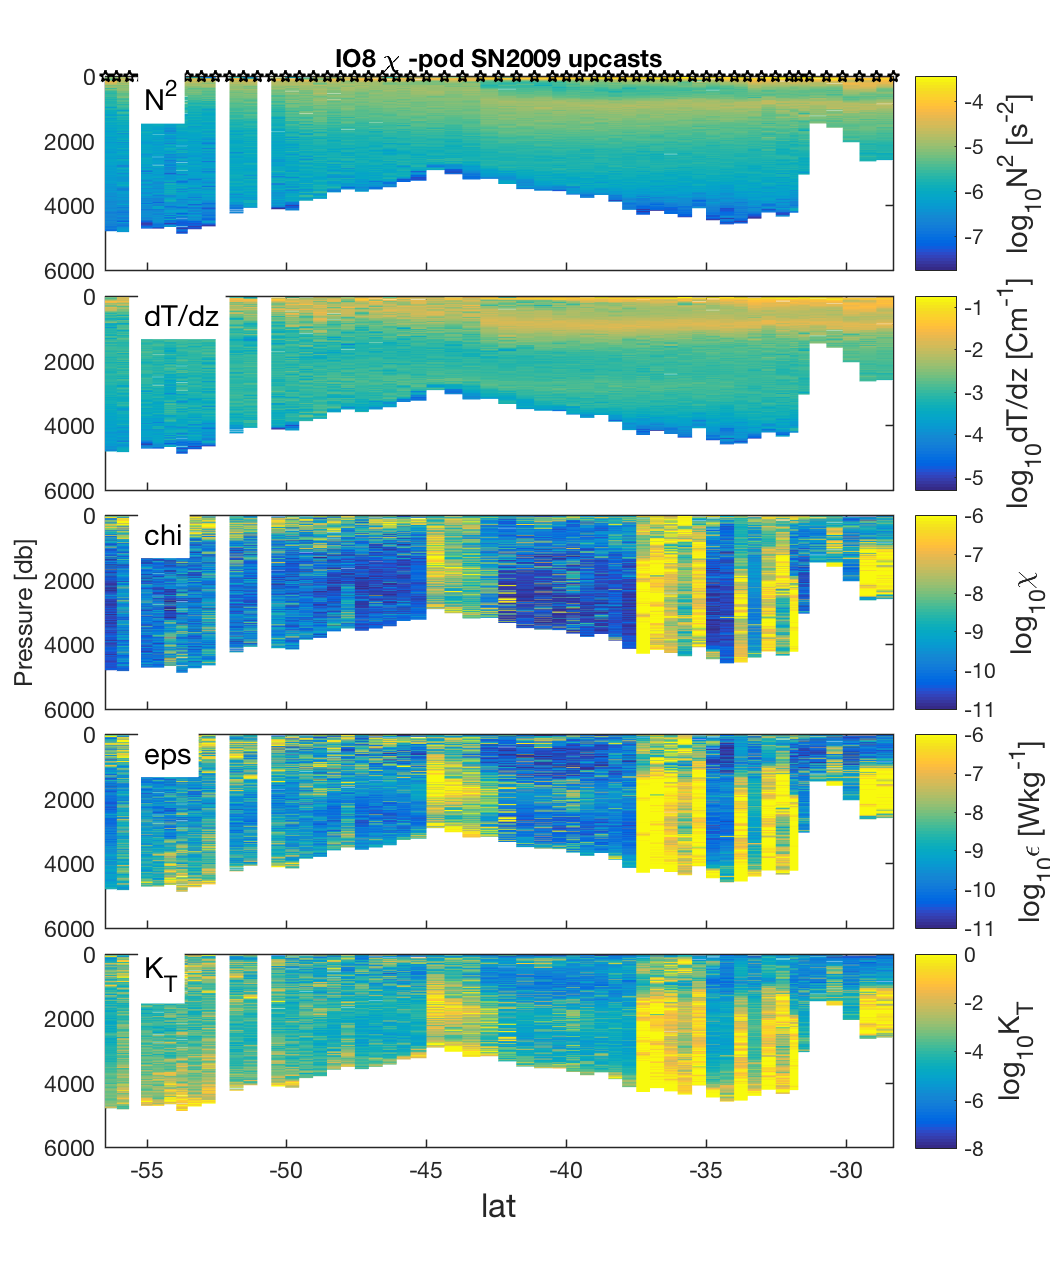
\includegraphics[scale=0.9]{XC_SN2009_Vs_lat_upAllVars.png}
\caption{All chipod profiles from sensor SN2009. Variables are: N2, dTdz, chi, eps, and KT.}
\label{}
\end{figure}

%~~~~~~~
\subsection{SN2020}

\begin{figure}[htbp]
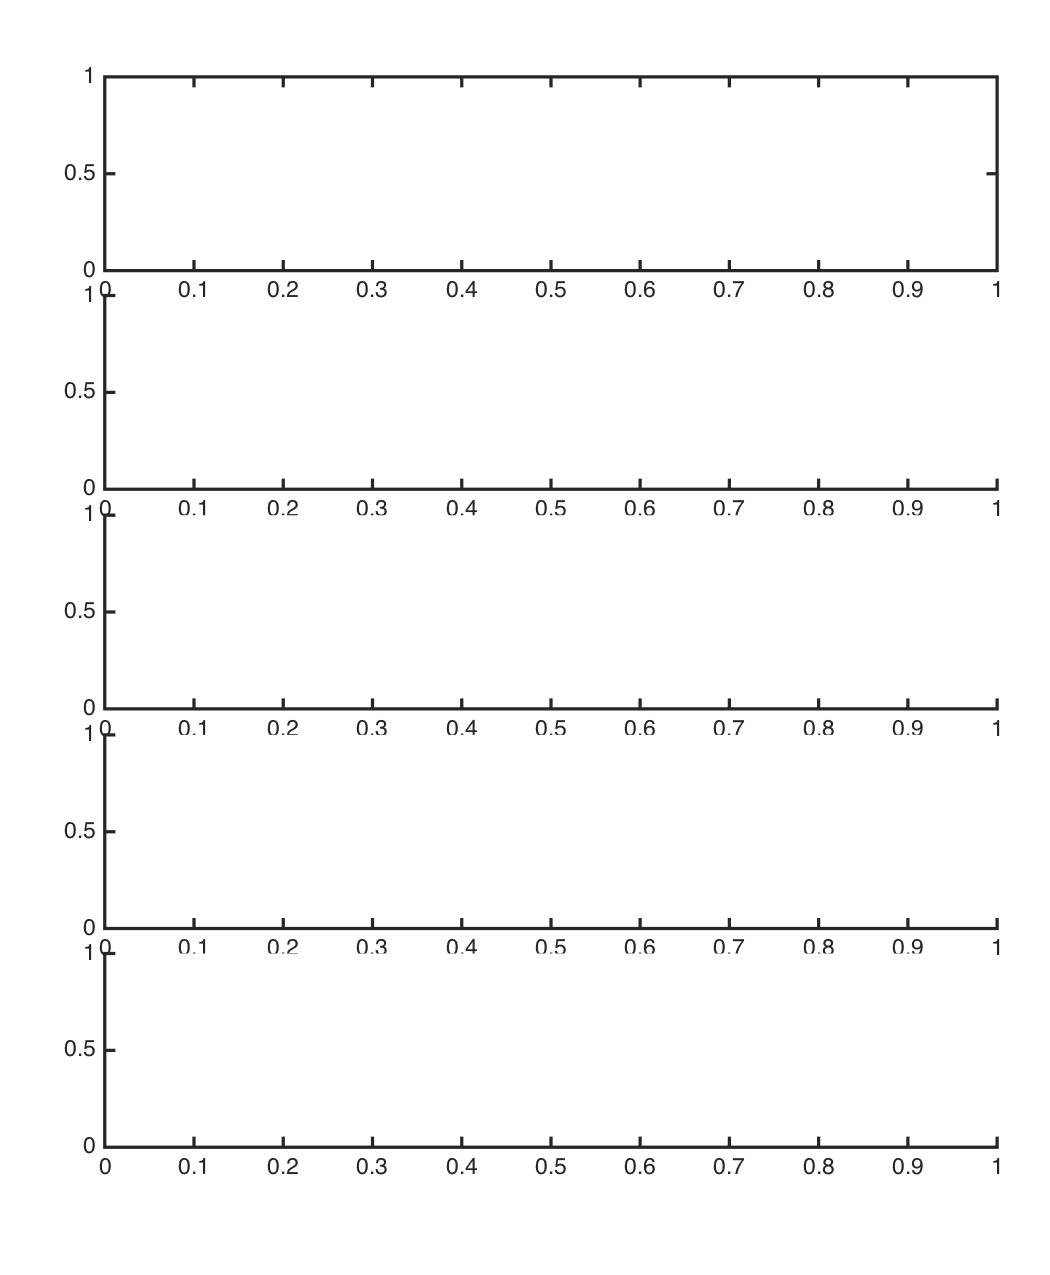
\includegraphics[scale=0.9]{XC_SN2020_Vs_lat_upAllVars.png}
\caption{All chipod profiles from sensor SN2020. Variables are: N2, dTdz, chi, eps, and KT.}
\label{}
\end{figure}



\clearpage
\newpage
%~~
\section{One variable from all Chipods}

\clearpage
%~~~~~
%\subsection{Before CTD lost}

\begin{figure}[htbp]
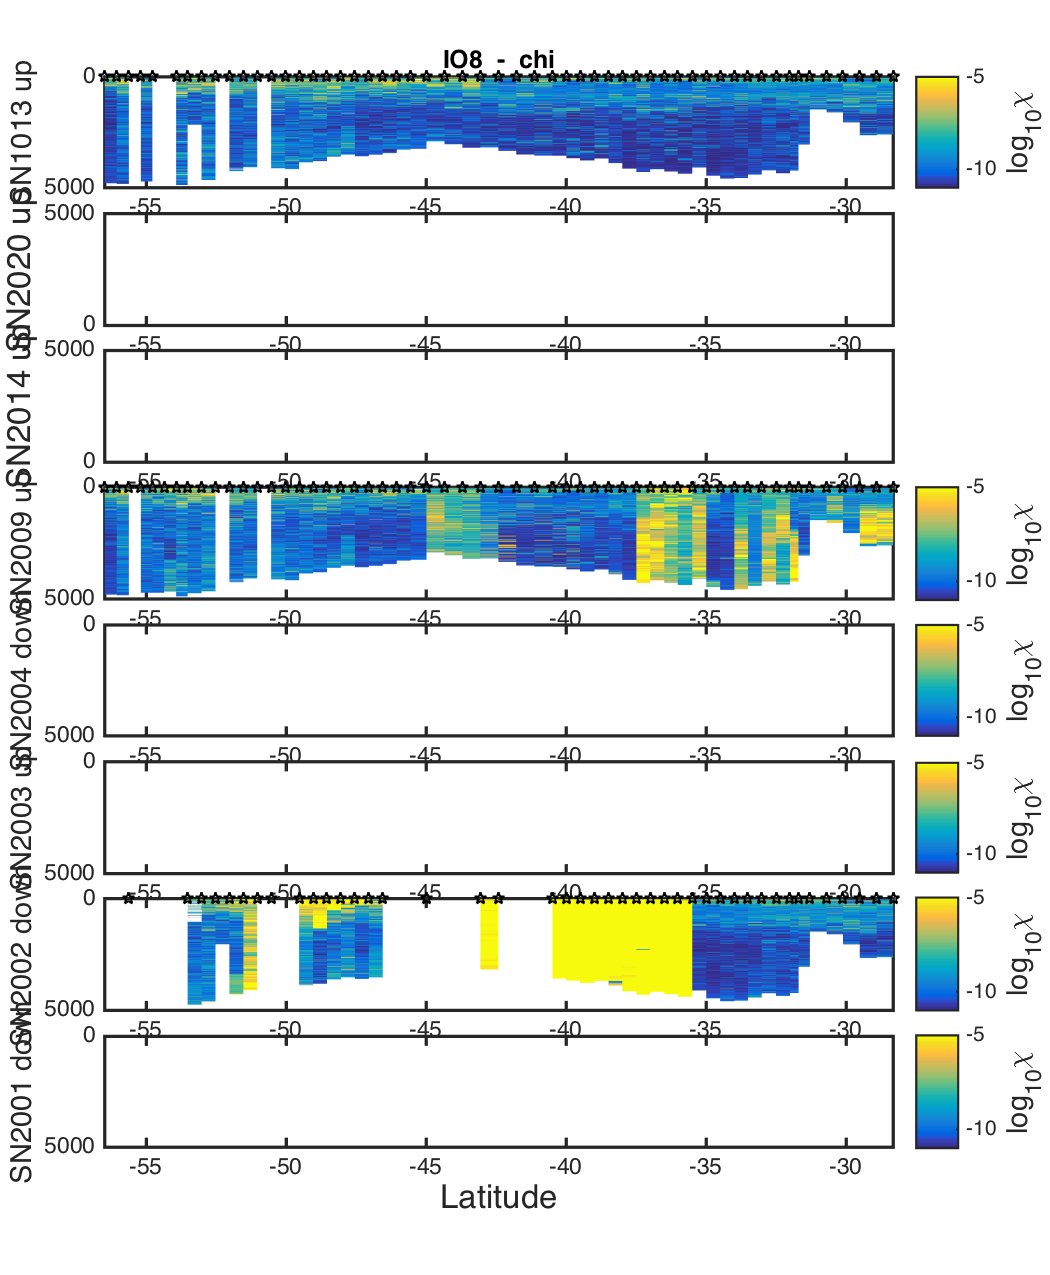
\includegraphics[scale=1]{IO8_chi_AllSNs_Vslat.png}
\caption{Plot of $\chi$ from 4 chipods on I08. These were the 4 units that were lost with the first CTD rosette.}
\label{}
\end{figure}


\begin{figure}[htbp]
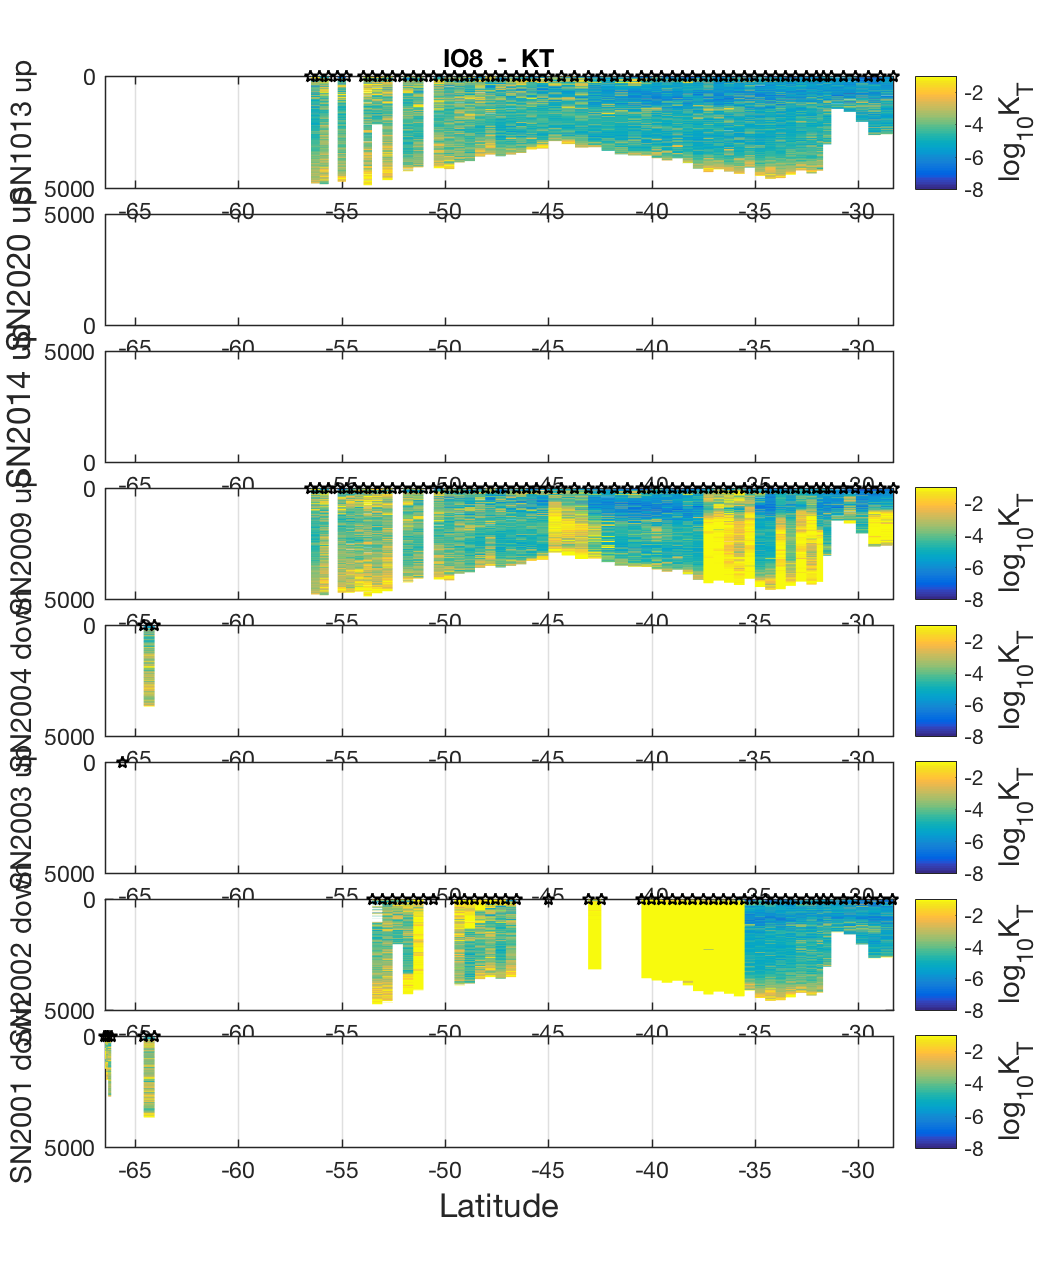
\includegraphics[scale=1]{IO8_KT_AllSNs_Vslat.png}
\caption{Plot of $K_T$ from 4 chipods on I08. These were the 4 units that were lost with the first CTD rosette.}
\label{}
\end{figure}

%
%\begin{figure}[htbp]
%\includegraphics[scale=1]{I08_chi_2020_2003_2004_2001.png}
%\caption{Plot of $\chi$ from 4 chipods on I08. These were the 4 units that were lost with the first CTD rosette.}
%\label{}
%\end{figure}
%
%\begin{figure}[htbp]
%\includegraphics[scale=1]{I08_chi_2020_2003_2004_2001.png}
%\caption{Plot of $K_T$ from 4 chipods on I08. These were the 4 units that were lost with the first CTD rosette.} CTD rosette.}
%\label{}
%\end{figure}
%
%
%\clearpage
%%~~~~~
%\subsection{After CTD lost}
%
%\begin{figure}[htbp]
%\includegraphics[scale=1]{I08_chi_1013_2009_2002.png}
%\caption{Plot of $\chi$ from 3 chipods on I08. These were the 3 units that returned most data after the loss of the first CTD rosette.}
%\label{}
%\end{figure}
%
%\begin{figure}[htbp]
%\includegraphics[scale=1]{I08_KT_1013_2009_2002.png}
%\caption{Plot of $K_T$ from 3 chipods on I08. These were the 3 units that returned most data after the loss of the first CTD rosette.}
%\label{}
%\end{figure}
%
%
%

%\newpage
%\clearpage
%\newpage
%%~~~~~~~~~~~~~~~~~~~~~~~~~~~~~
%\section{To-Do}
%
%\begin{itemize}
%\end{itemize}


%%~~~~~~~~~~~~~~~~~~~~~~~~~
% \bibliographystyle{ametsoc2014}
%\bibliography{/Users/Andy/Cruises_Research/wavechasers_bib/main}





\end{document}  
